\documentclass[
    bindingoffset=5mm,  % Binding offset
    footnoteindent=3mm, % Footnote indent
    hyphenation=true    % Hyphenation turn on/off
]{src/wut-thesis}

\graphicspath{{tex/img/}} % Katalog z obrazkami.
\addbibresource{report.bib} % Plik .bib z bibliografią
%-------------------------------------------------------------
% Wybór wydziału:
%  \facultyeiti: Wydział Elektroniki i Technik Informacyjnych
%  \facultymeil: Wydział Mechaniczny Energetyki i Lotnictwa
% --
% Rodzaj pracy: \EngineerThesis, \MasterThesis
% --
% Wybór języka: \langpol, \langeng
%-------------------------------------------------------------
\facultyeiti    % Wydział Elektroniki i Technik Informacyjnych
\langpol % Praca w języku polskim


%--------------
% Zmiana nazwy podpisów pod rysunkami
%--------------
\renewcommand{\figurename}{Rysunek}
\addto\captionspolish{\renewcommand{\figurename}{Rysunek}}
%\def\graphname{Wykres}
%\def\tablename{Tab.}

% Package options
\usetikzlibrary{automata, positioning}

\newcommand{\nodewidth}{0.449\textwidth}
\newcommand{\textnodewidth}{0.4\textwidth}

\begin{document}
%------------------
% Strona tytułowa
%------------------
\title{
Semantyczna analiza środowiska\\
przez robota usługowego\\ \vspace{1cm}  
Sprawozdanie
}
\author{Piotr Hondra}
\date{\the\year}
\maketitle

%--------------
% Spis treści
%--------------
% \cleardoublepage % Zaczynamy od nieparzystej strony
\clearpage
\tableofcontents

%------------
% Rozdziały
%------------
% \cleardoublepage % Zaczynamy od nieparzystej strony
\clearpage
\pagestyle{headings}

% Wygodnie jest trzymać każdy rozdział w osobnym pliku.
% Umożliwia to również łatwą migrację do nowej wersji szablonu:
% zazwyczaj wystarczy podmienić plik src/wut-thesis.cls
%\input{tex/1-cos}
\section{Wstęp teoretyczny}
\subsection{Klasyfikacja sceny}
\begin{figure}
    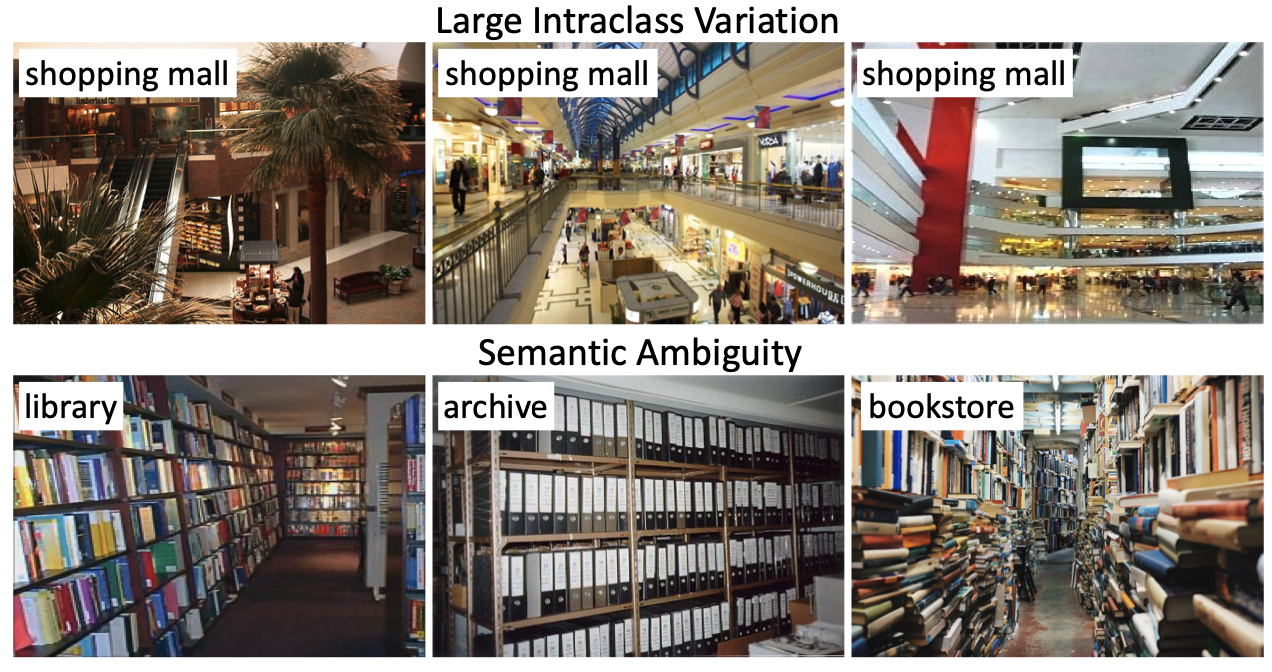
\includegraphics[width=\textwidth]{images/scene_class.png}
    \caption{Problem różnorodności wewnątrzklasowej oraz wieloznaczności semantycznej \cite{zeng2021deep}.}
    \label{fig:scene-class}
\end{figure}

Zadanie klasyfikacji sceny polega na przyporządkowaniu kategorii miejsca, w które przedstawia obraz. Istnieje duża różnica między klasyfikacja obrazka a klasyfikacją sceny. Klasyfikacja obrazka jako taka zajmuje się przyporządkowaniem klasy obiektu pierwszoplanowego, np. czy na obrazie znajduje się pies, czy kot. Klasyfikacja sceny natomiast musi wziąć pod uwagę wszystkie cechy obrazu, zarówno tła, jak i pierwszego planu, by określić odpowiednie miejsce.

Zadanie klasyfikacji sceny jest trudne ze względu na problem różnorodności wewnątrz klasowej oraz wieloznaczności semantycznej, co zostało przedstawione na rys. \ref{fig:scene-class}. Pierwszy z nich polega na fakcie, iż jedno miejsce może zostać przedstawione w bardzo różnej konfiguracji m.in. oświetlenia, ekspozycji, obiektów znajdujących się na obrazie. Drugi jest związany z występowaniem tych samych obiektów dla różnych klas scen.

\subsection{Segmentacja obrazu}
\begin{figure}
    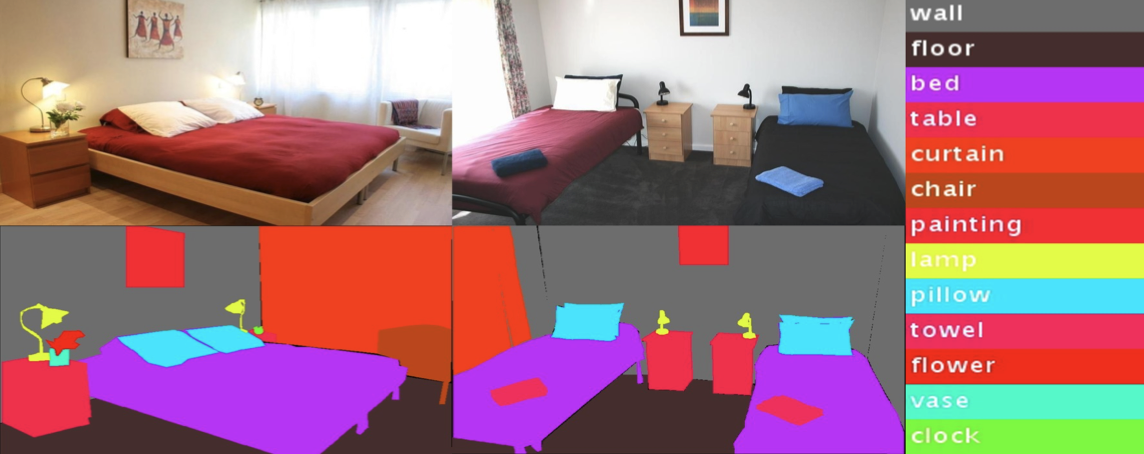
\includegraphics[width=\textwidth]{images/segment.png}
    \caption{Segmentacja wewnątrz pomieszczeń \cite{zhang2018context}.}
    \label{fig:segment}
  \end{figure}

Zadanie segmentacji obrazu to przyporządkowanie każdemu pikselowi etykiety (rys. \ref{fig:segment}). W rezultacie obraz zostaje podzielony na homogeniczne regiony pod względem pewnych własności.

\section{Cel pracy}
Celem pracy inżynierskiej są dwa zadania:
\begin{itemize}
    \item segmentacja środowiska wewnątrz budynku
    \item klasyfikacja pomieszczeń
\end{itemize}
\section{Założenia}
Praca zakłada wykonanie celów pracy w środowisku wewnątrz budynków, co więcej będzie to środowisko domowe. Ponadto inferencja zostanie przeprowadzona na robocie Tiago, który jest wyposażony w kamerę Kinect.
\section{Motywacje}
Istnieje wiele powodów, dla których temat pracy jest wart uwagi.

Po pierwsze rozwiązanie może być wykorzystane w nawigacji robota. Wykrywanie przeszkód jest kluczowym aspektem możliwości poruszania się robota. Zostanie ono podjęte przez zadanie segmentacji. Należy zwrócić uwagę, że robot powinien zachowywać się ostrożniej w kuchni oraz w łazience. Ta informacja zostanie uzyskana poprzez klasyfikację sceny.

Innym zastosowanie rozważanego rozwiązania jest pomoc dla osób niewidomych. Osoba niepełnosprawna mogłaby wówczas poruszać się po środowisku domowym z większą łatwością, mając na sobie kamerę oraz informację o otaczającej przestrzeni.

\section{Zbiór danych}

Zbiór danych powinien ściśle odpowiadać założeniom postawionym w pracy. Inferencja wymaga użycia kamery Kinect. Zatem zbiór danych powinien zawierać kategorie scen, segmentacje obrazów oraz najlepiej być ujętym przez kamerę Kinect wersji pierwszej.

Po prześledzeniu wielu zbiorów danych udało się sprostać powyższym wymaganiom, uzyskując dwa podobne zbiory danych.

\begin{table}[]
    \begin{adjustbox}{width=\columnwidth,center}
    \begin{tabular}{l|ccccccc}
    Nazwa    & \# Ilość & \# Klas obiektów & \# Klas scen & RGB-D     & Rozdzielczość & \# Czujników & Nieposprzątane \\ \hline \hline
    NYUv2    & 1 449    & 894              & 26           & \checkmark & 640 x 480     & 1            & \checkmark                   \\
    SUN RGBD & 10 335   & 800              & 47           & \checkmark & 640 x 480     & 4            & x                         
    \end{tabular}
    \end{adjustbox}
    \caption{Porównanie zbiorów danych \cite{song2015sun},\cite{silberman2012indoor}}
    \label{tab:dataset}
\end{table}

Porównanie zbiorów \texttt{NYUv2} oraz \texttt{SUN RGBD} przedstawiono w tabeli \ref{tab:dataset}. Mimo liczbowej przewagi \texttt{SUN RGBD} pod wieloma względami ostatecznie wybrano \texttt{NYUv2} z uwagi, że zbiór ten został zebrany dla pomieszczeń, w które nie są posprzątane. Fakt ten uznano, za kluczowy, iż uważano, że będzie przekładał się na lepsze rezultaty w naturalnych warunkach. \texttt{NYUv2} jest też chętniej cytowany niż texttt{SUN RGBD} (rys. \ref{fig:sun-vs-nyu}).

\begin{figure}
    \centering
    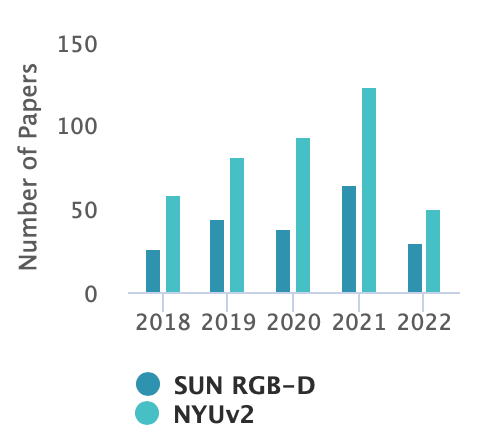
\includegraphics[width=0.5\textwidth]{images/stats-dataset.png}
    \caption[]{Szacowana liczba cytowań w latach 2018-2022 \href{https://paperswithcode.com/dataset/sun-rgb-d}{[paperswithcode.com]}}
    \label{fig:sun-vs-nyu}
\end{figure}

\section{Przegląd rozwiązań}
\subsection{Metody klasyczne}
\begin{figure}
    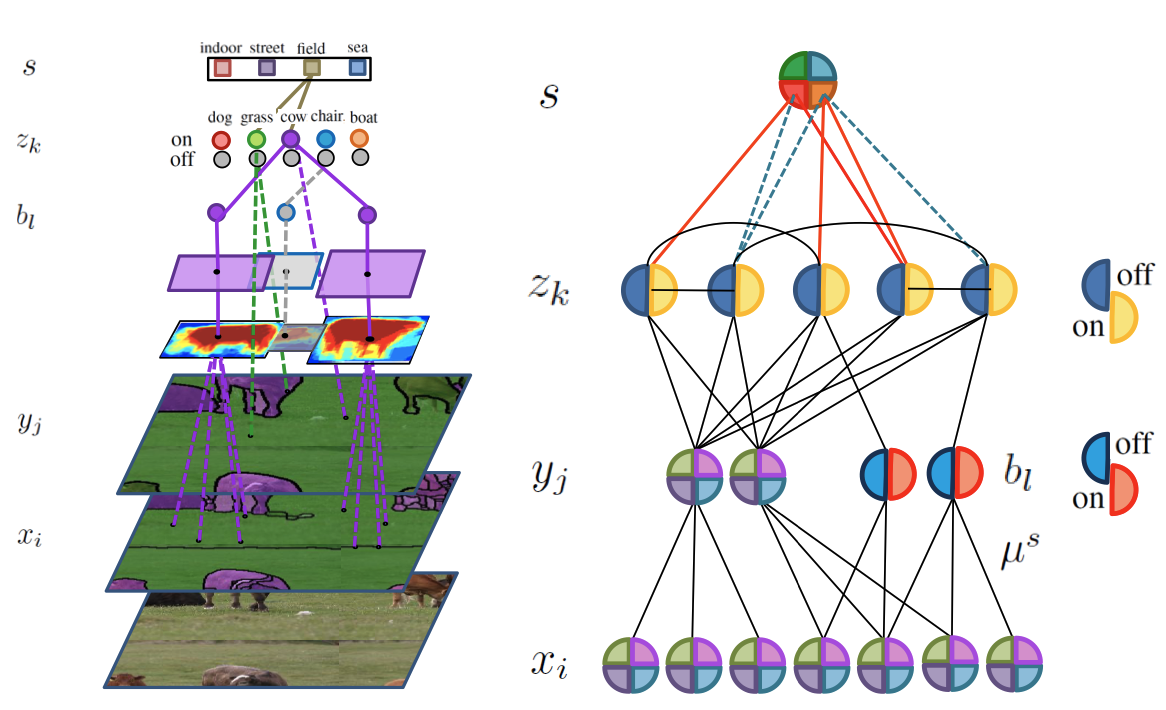
\includegraphics[width=\textwidth]{images/joint-segmentation-and-classification.png}
    \caption{Describing the Scene as a Whole: Joint Object Detection, Scene Classification and Semantic Segmentation 2012 \cite{yao2012describing}.}
    \label{fig:old-school-arch}
\end{figure}

Artykuł ,,Describing the Scene as a Whole: Joint Object Detection, Scene Classification and Semantic Segmentation 2012 \cite{yao2012describing}'' dobrze ilustruje relacje segmentacji obrazu oraz klasyfikacji sceny. Aby odpowiednio sklasyfikować scenę, należy obraz przedstawić w postaci cech, a następnie na tej podstawie dopiero wnioskować. Artykuł \cite{yao2012describing} udowadnia, iż możliwe jest przeprowadzenie wnioskowania na podstawie segmentacji (rys. \ref{fig:old-school-arch}).

\subsection{Metody oparte o głębokie uczenie}

\begin{figure}
    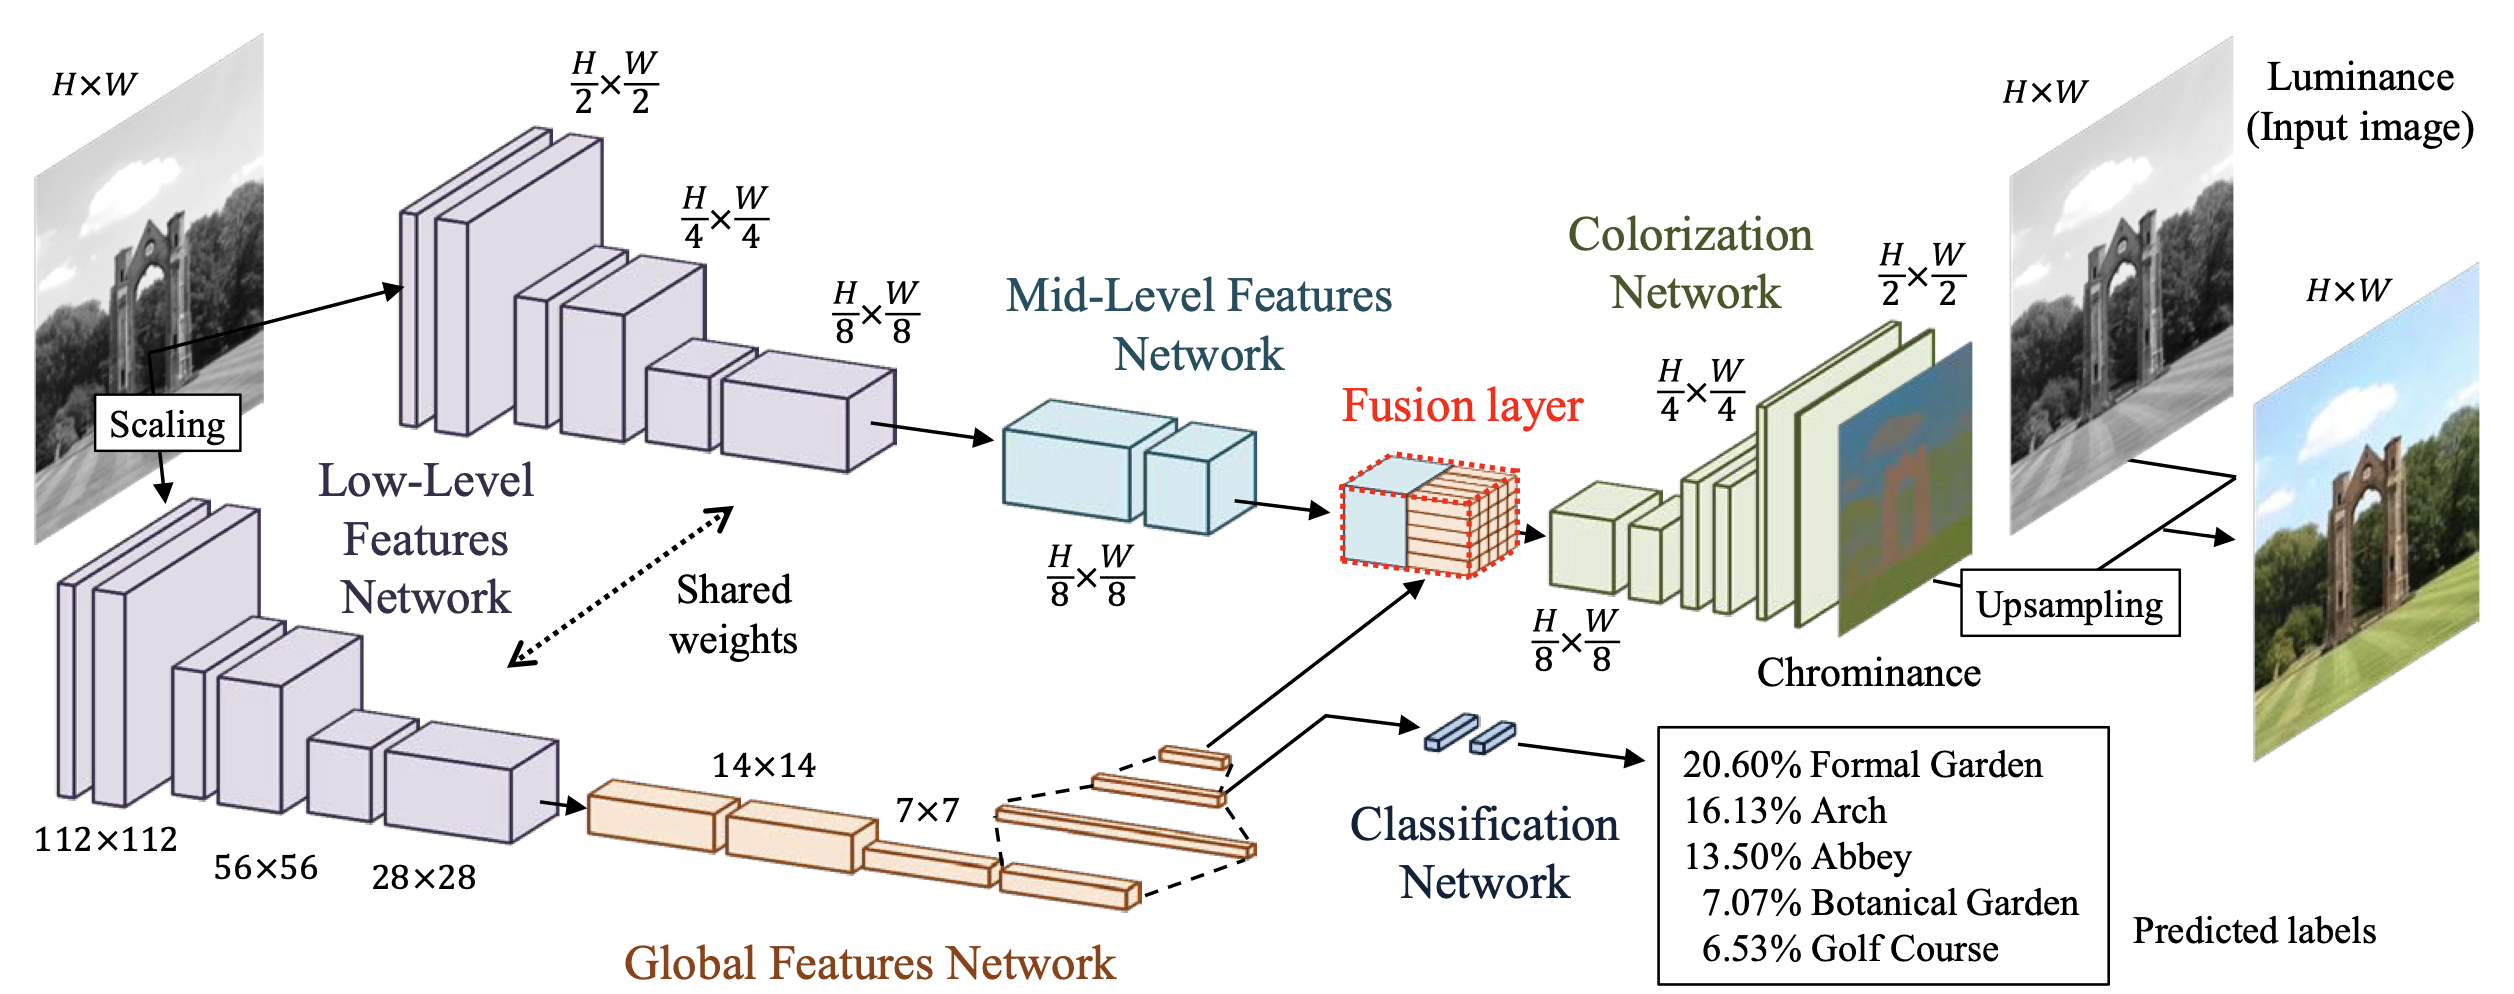
\includegraphics[width=\textwidth]{images/global-local-features.png}
    \caption{Let there be Color!: Joint End-to-end Learning of Global and Local Image Priors for Automatic Image Colorization with Simultaneous Classification 2016 \cite{iizuka2016let}.}
    \label{fig:parrarel-arch}
\end{figure}

Współcześnie do zadań wizji komputerowej używa się głębokich sieci neuronowych z uwagi na ich duże zdolności generalizacji skomplikowanych przestrzeni. Celem każdej architektury jest odpowiednia ekstrakcja cech w sposób łatwo ekstrahowalny. Architektury różnią się zatem sposobem generalizacji, a dokładniej ułożeniem warstw i ich parametrów. W ramach przeglądu literatury pochylono się nad różnymi metodami łączenia zadania segmentacji i klasyfikacji, ponieważ zadanie postawione w pracy, co do wiedzy autora, nie zostało wcześniej rozwiązane podobnymi metodami.

Pierwszy artykuł ,,Let there be Color!: Joint End-to-end Learning of Global and Local Image Priors for Automatic Image Colorization with Simultaneous Classification 2016 \cite{iizuka2016let}'' rozwiązuje problem kolorowania obrazków jednak, przekształcony może być użyty w pracy. Tego można dokonać odrzucając ostatnią warstwę konkatenacji w części segmentacji (rys. \ref{fig:parrarel-arch}). Przedstawiona architektura symultanicznie ekstrahuję cechy globalne oraz średniego poziomu, które odpowiednio służą klasyfikacji oraz segmentacji.

\begin{figure}
    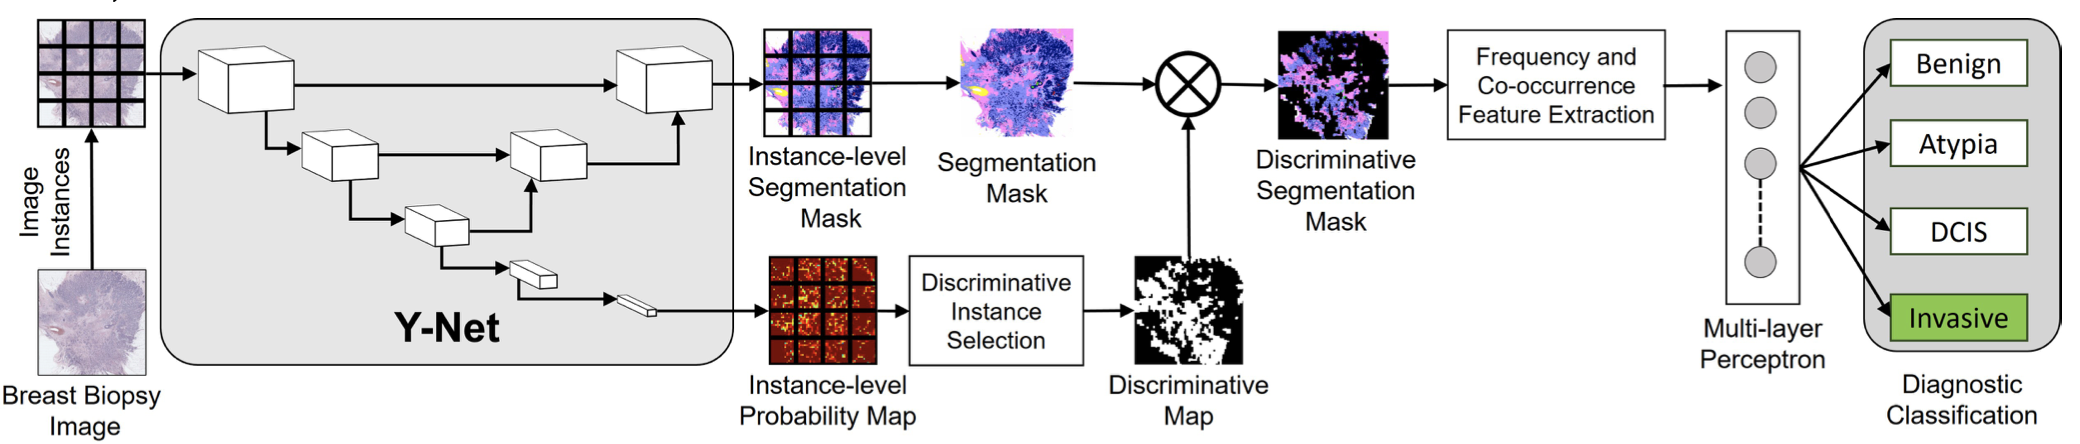
\includegraphics[width=\textwidth]{images/y-net.png}
    \caption{Y-Net: Joint Segmentation and Classification for Diagnosis of Breast Biopsy Images 2018 \cite{mehta2018net}.}
    \label{fig:y-net}
\end{figure}

Kolejnym artykułem jest ,,Y-Net: Joint Segmentation and Classification for Diagnosis of Breast Biopsy Images 2018 \cite{mehta2018net}''. Jest to standardowa architektura segmentacji \texttt{U-Net} rozszerzona o gałąź klasyfikacyjną (rys. \ref{fig:y-net}). Rozwiązanie to jest na pewno ciekawe z punku widzenia modularności rozwiązania.

\section{Zaproponowane rozwiązanie}
\begin{figure}[h]
    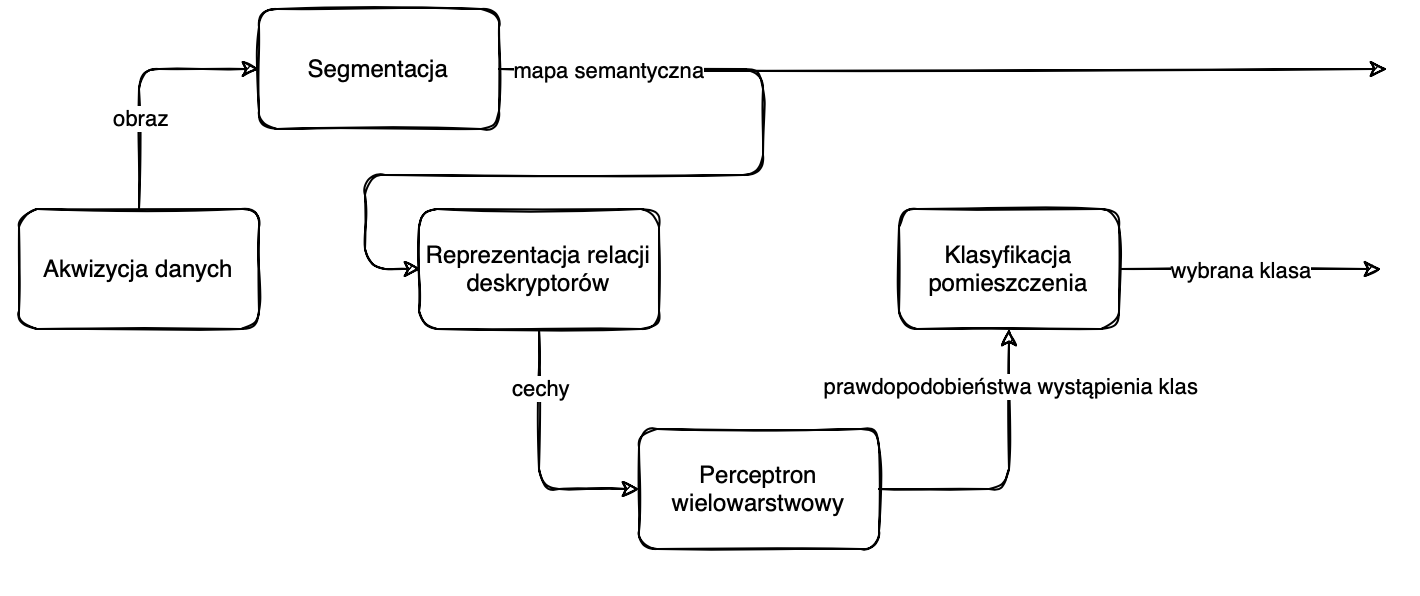
\includegraphics[width=\textwidth]{images/own-solution.png}
    \caption{Prototyp rozwiązania.}
    \label{fig:prototype}
\end{figure}
W swoim rozwiązaniu chciałbym wykorzystać głębokie sieci neuronowe do realizacji celów pracy. Proponuję jako prototyp wykorzystać segmentację jako reprezentację cech wysokiej abstrakcji. Następnie na podstawie relacji opisanych wyżej cech zbudować klasyfikator w formie perceptronu wielowarstwowego. Na wyjściu zgodnie z rysunkiem \ref{fig:prototype} otrzymać mapę semantyczną oraz klasyfikację scen.

W kolejnych iteracjach pracy chciałbym zbudować inne architektury, a ostatecznie porównać je, wybierając architekturę o największej skuteczności.

 % Można też pisać rozdziały w jednym pliku.
%\clearpage % Zawsze zaczynamy rozdział od nowej strony

%---------------
% Bibliografia
%---------------
\cleardoublepage % Zaczynamy od nieparzystej strony
\printbibliography

%--------------------------------------
% Spisy: rysunków, tabel, załączników
%--------------------------------------
\clearpage
\pagestyle{plain}

\listoffigurestoc    % Spis rysunków.
%\vspace{1cm}         % vertical space
%\listoftablestoc     % Spis tabel.
%\vspace{1cm}         % vertical space
%\listofappendicestoc % Spis załączników

% Wykaz symboli i skrótów.
% Pamiętaj, żeby posortować symbole alfabetycznie
% we własnym zakresie. Makro \acronymlist
% generuje właściwy tytuł sekcji, w zależności od języka.
% Makro \acronym dodaje skrót/symbol do listy,
% zapewniając podstawowe formatowanie.
%\vspace{0.8cm}
%\acronymlist
%\acronym{EiTI}{Wydział Elektroniki i Technik Informacyjnych}
%\acronym{PW}{Politechnika Warszawska}

%-------------
% Załączniki
%-------------

% Obrazki i tabele w załącznikach nie trafiają do spisów
%\captionsetup[figure]{list=no}
%\captionsetup[table]{list=no}

% Używając powyższych spisów jako szablonu,
% możesz dodać również swój własny wykaz,
% np. spis algorytmów.

\end{document} % Dobranoc.
